%% ------------------------------------------------------------------------- %%
\chapter{Research Methodology}
\label{cap:research}

 \epigraph{
 Work it harder, make it better,\\
 Do it faster, makes us stronger,\\
 More than ever, hour after hour,\\
 Work is never over.}
 {Daft Punk}

\paragraphdesc{description of the research: qualitative and quantitative}
This research was conducted following quantitative and qualitative approaches.
The quantitative approach evaluated the technologies selected for the experiments, while the qualitative approach gathered data from applications' users.
Data was analyzed and used as basis for improvements of applications, based on users expectations.

\paragraphdesc{remember goals: this is where you want to go}
The primary goal of this research, as stated in the first chapter, is to evaluate the current technologies and trends for mobile interaction, whereas 
a secondary goal is to promote the use of mobile technologies by musicians and artists, even without technical knowledge.
These goals seek to bridge the gaps identified in mobile music practices, targeting those who intend to use network technologies and mobile devices for collaborative and cooperative interaction during music performances.


\paragraphdesc{how to define the paths that lead to the goals (this is the methodology!)}
\paragraphdesc{evaluate mobile technologies in/for performances}
To accomplish these goals, applications were developed to provide working solutions for specific scenarios in mobile music, and experiments were conducted to map possibilities and difficulties found in such scenarios.
The applications developed during this research have their description at Appendix~\ref{ape:applications}, following a chronological order that reflects the research process.
Chapter~\ref{cap:evaluations} presents the network technologies evaluation along with discussions of the use of these technologies and identified constraints.
Technology evaluation follows two patterns. 
Some evaluation target the automatic exploration of different parameters used in mobile music interaction, different services and routing schemes, and data gathered over long periods of time.
Papers, talks, demonstrations, installations, and performances are the means to accomplish the secondary goal.
Papers, published and presented at several computer music conferences in Brazil and abroad, offered opportunities to reach researchers, musicians, and lay audiences interested in mobile music.
These papers were included in this thesis as Appendix~\ref{ape:papers}

\paragraphdesc{methodologies of past projects from compmus: inspire, cooperate, collaborate}
During the development of this project, other related projects were developed by members of the computer music research group at IME/USP, whose methodologies also were considered in this study.
André Bianchi's study of mobile platforms for realtime audio processing produced the \textit{DSPBenchmarking}~\citep{Bianchi2012ontheperformance}, an open source application for Android DSP evaluation.
A partnership with André Bianchi allowed evaluations of DSP techniques that outperform traditional approaches, as presented in detail in Appendix~\ref{apesec:appdspbenchmarking}.
Flávio Schiavoni developed \textit{Medusa}~\citep{Schiavoni2011medusa}, an open source tool for network distributed performances with audio and MIDI.
In Flávio's research, network tests using the loopback approach were conducted in order to calculate RTT between computers using different network transport protocols; this methodology was adapted to be used here with mobile devices and different services and routing schemes.

\paragraphdesc{organic research: study, experiment, innovate}
This thesis is also the result of an organic research methodology focusing on alternating periods of studies, experimentation, and innovation.
Periods of studies through courses and books were carried out before the first experiments with each technology addressed, leading to pilot experiments viewed as learning tools.
Issues and alternatives that appeared during these experiments turned out to be valuable resources for periods of brainstorms leading to innovations in the strategies implemented.
To propose innovative solutions, and to try them out by developing software, were stepstones of the research methodology that helped identifying gaps and shortcomings, which demanded new studies, leading to new research cycles.

\paragraphdesc{research plan #1: evaluate current options}
\paragraphdesc{research plan #2: evaluate (possible) future options}
The explorative investigation of technologies for mobile music may be categorized in two main branches or research plans.
The first research plan focused on the evaluation of currently explored options from the mobile music state-of-the-art, as found in existing literature.
Appendix~\ref{ape:applications} offers a comprehensive description of this first research plan containing the steps dealt with in detail.
A second research plan is based on exploring options for mobile music from trending mobile technologies that are unpopular or little widespread in mobile music scenarios. 
These include newer technologies such as IPv6 and gigabit connections, that will be broadly available in the future but aren't yet at the time and place where this research was conducted, and also technologies that were available but didn't yet make their way into mobile music projects, such as Multicast routing and Cloud Services.

%%%%%%%%%%%%%%%%%%%%%%%%%%%%%%%
\section{Methodology for exploring mobile devices in mobile music}

\paragraphdesc{Android and iOS options}
The focus of this research are mobile devices, especially smartphones.
Exploring mobile devices in real concert situations was the aim of many installations and performances conceived and carried out during this research process.
Bearing this in mind, and also the availabity of specific devices within the collaborating research groups, most devices used during application development were Android-based, whereas iOS devices where used in specific partnerships.
Other devices were also used in this research by audiences during web-based collaborative and distributed performances which would only require Internet access. 

\paragraphdesc{open/closed source code evaluation for free: git (open source) or APK (closed source)}
The Android operating system was selected as the main focus for application development during this research for some reasons, one of them being the ease of adopting FLOSS ideals in development.
Applications were developed under free licenses with open sources and became available for use through Github repositories, F-Droid, and compiled applications. On one hand, source-based distribution is useful for collaborative development, and on the other hand distribution of compiled versions (apk) is more friendly to interested users and beta testers.
Android also offers possibility of distributing applications through Bluetooth, WiFi, or web pages, without the burden of having to publish them or sign provisioning profiles with a device ID as in the case of iOS applications.

\paragraphdesc{development with Eclipse + ADT}
\paragraphdesc{development with Android Studio}
Android application development was based in two main IDEs.
The Eclipse IDE was used during the development of the first applications, mainly due to its popularity among Android developers.
This IDE requires the Android Development Tools~(ADT) plugin for compiling applications and communicating with Android devices and emulators.
By the end of the research period, the Eclipse ADT became deprecated and the application development moved on to Android Studio.
Android Studio is the official IDE for the development of Android applications and replaced the Eclipse ADT by the end of 2015\footnote{An update on Eclipse Android Developer Tools - Android Developers Blog: \url{https://android-developers.googleblog.com/2015/06/an-update-on-eclipse-android-developer.html} (visited on May, 2017)}.
This IDE presents a complete environment offering many tools for debugging and monitoring running applications.

\paragraphdesc{application testing with emulators (why not)}
Emulators allowed running applications together with the IDEs inside the same machine.
This option facilitates interface design and local network simulation.
The emulators used during this research were based on the native images that come with the Android SDK, and also the Genymotion Android Emulator\footnote{Genymotion Android Emulator website: \url{https://www.genymotion.com/} (visited on May, 2017)}.
Although Android emulators can simulate virtual sensors at their current versions, some applications required the evaluation of sensors and other features unavailable at emulators during the development period and obliged the use of real devices as well.

\paragraphdesc{real devices for testing: devices used during research}
The mobile devices used during evaluations were LG D686 G Pro Dual Lite, Samsung GT-I9300 Galaxy SIII, and Sony Xperia D8533/D8503 Z3 Compact, abbreviated as D686, S3, and Z3, respectively.
Their main technical specifications are presented on the Table~\ref{tab:gsmarena-lg-s3-z3-short}, and the complete settings of the devices are described in Appendix~\ref{ape:gsmarena-lg-s3-z3}.
Additionally, many uncatalogued personal devices were used during the application development process (by beta testers) and also during the installations (by the audiences).

\begin{longtable}{llp{0.2\linewidth}p{0.2\linewidth}p{0.2\linewidth}}
	\caption{Main technical specifications of the mobile devices used during evaluations: D686, S3, and Z3. Source: Adapted from \cite{GSMARENA2017-lg-s3-z3}} \\ \hline
	&               & LG D686 G Pro Lite Dual                              & Samsung GT-I9300 Galaxy SIII                                                                  & Sony D8533 (and D8503) Xperia Z3 Compact                                                          \\ \hline \endhead
	LAUNCH   & Announced     & 2013, October                                   & 2012, May                                                                                   & 2014, September                                                                                                \\
	& Status        & Available. Released 2013, November              & Available. Released 2012, May                                                               & Available. Released 2014, September                                                                            \\ \hline
	PLATFORM & OS            & Android OS, v4.1.2 (Jelly Bean)                 & Android OS, v4.0.4 (Ice Cream Sandwich), 4.3 (Jelly Bean)                                   & Android OS, v4.4.4 (KitKat), upgradable to v6.0 (Marshmallow)                                                  \\
	& Chipset       & Mediatek MT6577                                 & Exynos 4412 Quad                                                                            & Qualcomm MSM8974AC Snapdragon 801                                                                              \\
	& CPU           & Dual-core 1.0 GHz Cortex-A9                     & Quad-core 1.4 GHz Cortex-A9                                                                 & Quad-core 2.5 GHz Krait 400                                                                                    \\
	& GPU           & PowerVR SGX531                                  & Mali-400MP4                                                                                 & Adreno 330                                                                                                     \\ \hline
	MEMORY   & Card slot     & microSD, up to 32 GB (dedicated slot)           & microSD, up to 64 GB (dedicated slot)                                                       & microSD, up to 256 GB (dedicated slot)                                                                         \\
	& Internal      & 8 GB, 1 GB RAM                                  & 16/32/64 GB, 1 GB RAM                                                                       & 16 GB, 2 GB RAM                                                                                                \\ \hline
	COMMS    & WLAN          & Wi-Fi 802.11 b/g/n, Wi-Fi Direct, DLNA, hotspot & Wi-Fi 802.11 a/b/g/n, dual-band, Wi-Fi Direct, DLNA, hotspot                                & Wi-Fi 802.11 a/b/g/n/ac, dual-band, Wi-Fi Direct, DLNA, hotspot                                                \\
	& Bluetooth     & v3.0, A2DP                                      & v4.0, A2DP, EDR, aptX                                                                       & v4.0, A2DP, LE, aptX                                                                                           \\ \hline
	FEATURES & Sensors       & Accelerometer, proximity, compass               & Accelerometer, gyro, proximity, compass, barometer                                          & Accelerometer, gyro, proximity, compass, barometer                                                             \\ \hline
	\label{tab:gsmarena-lg-s3-z3-short}
\end{longtable}

\paragraphdesc{iOS}
\paragraphdesc{\textit{urMus}}
Some applications for iOS devices using the \textit{\textit{urMus}} platform~\citep{Kim2011urmus} were developed during the period as an exchange student at the University of Michigan under the supervision of Professor Georg Essl.
Within Professor Essl's group many iOS devices, such as iPods, iPhones, and iPads, were available for research purposes.
All of these devices had the \textit{urMus} platform installed and this allowed the development of mobile music applications without the need of subscribing to the Apple Developer Program.
A web interface for the \textit{urMus} platform  is available, which allows developers to deploy new codes and interfaces for mobile applications.
The developed applications were tested on real devices and some of them were used during mobile performances by students.
The main evaluation of these applications was made through qualitative reports during demonstrations and rehearsals, and also from feedback by Professor Essl before performances.

\paragraphdesc{web technologies}
Some technologies such as PhoneGap\footnote{Adobe PhoneGap website: \url{https://phonegap.com/} (visited on December, 2018)} allow the development of hybrid solution using web technologies, where the same application runs on both Android and iOs devices without many modifications.
During this research process, the main web technology used for hybrid application development was Audio Synthesis with Web Audio and network communication through Cloud Services.
The compatibility of the Web Audio API with browsers available for several mobile platforms allows the participation of many users in a mobile music performance without the burden of having to install OS dependent applications, since all interaction and control is done within a web site.


%%%%%%%%%%%%%%%%%%%%%%%%%
\section{Network settings}

\paragraphdesc{Intranet and Internet alternatives}
Intranet and Internet were used in order to evaluate network alternatives for mobile music interaction and collaboration.
Some network communication options were available only in specific scenarios during the research and the applications evaluated through these solutions aimed to explore most of the available settings.
The comparison of alternative mobile technologies was conducted under similar conditions whenever possible (i.e. when technologies could be employed in similar scenarios).

\paragraphdesc{Local network}
Intranet setting evaluations were related to protocol options and other technical aspects.
Most of the evaluations using local networks were made using UDP for packet exchanging between Android devices and through Bonjour\footnote{Bonjour website: \url{https://support.apple.com/bonjour} (visited on December 2018)} for iOS.
An additional evaluation was made using the network infrastructure available for academic institutions, which might be considered an Intranet due to its private access policy and backbone topology.

\paragraphdesc{Academic Networks}
Academic institutions are usually connected through national networks which are in turn connected to other backbone networks in different countries.
Brazilian National Research and Educational Network~(RNP) manages the academic network available for Brazilian universities, while the Internet2 is responsible for interconnecting US universities, and RedCLARA is a network that interconnects Latin American academic networks.
These interconnected backbone networks were used in this research in order to evaluate long distance communication between Brazil and US.
This academic network allows the use of their services and also offers public IPs for devices.
Due to their private access, the use of these networks was only made possible after registering the research project within the academic network managerial infrastructure.

\paragraphdesc{Internet}
Use of the Internet was an expected approach since this technology is widely accessible.
Although many applications were designed for direct communication, some of them were designed to use Internet technologies such as web services and Cloud Services. These are interesting alternatives accessible to lay audiences and non-academic researchers as well.

\subsection*{Web service}
 
\paragraphdesc{web server as first alternative}
A web service was considered as the first option for evaluating the use of solutions for mobile music interaction over the Internet, since
using a web server for web service deployment is a common approach for web developers that want to distribute data between many devices and platforms.
A web server allows the creation of an online application on a shared computer that can be reached by anyone connected to the Internet.

\paragraphdesc{POST and GET approach}
The traditional HTTP requests, GET and POST, are common options available in APIs developed for web services.
During an interactive performance, the applications are expected to GET the most updated data and POST updated data in order to share with other devices, so the idea of focusing only on these requests was a natural approach for real-time interaction.
Other requests such as UPDATE or DELETE are less useful in a real time context where data is immediately used after it is shared, unless the user need to manage previously exchanged data afterwards.

\paragraphdesc{Ruby on Rails}
Web service development with an API can be hard for users without technical knowledge.
Bearing this in mind, a Rapid Application Development~(RAD) approach was an interesting alternative for exploration.
The Ruby on Rails~(RoR) framework\footnote{Ruby on Rails framework website: \url{https://rubyonrails.org/} (visited on December, 2018)} was selected to create the web application that would run on the web server and offer the required web services for exchanging data between mobile devices.
This framework offers the possibility of creating applications with just a few lines of code, describing the data that will be exchanged and the fields and types of database elements.
This framework is also an alternative for developers who intend to create complete multi-featured web applications without having to create their code from scratch based on a full Model View Controller~(MVC) design pattern.

\paragraphdesc{JSON}
An application created with RoR offers ready-to-use requests for getting, posting, updating, and deleting data, including support for widely-used data formats such as JSON.
This format was used in many applications developed during this research process due to its improved readability and cross-compatibility in comparison to alternatives such as XML.

\paragraphdesc{deploy at Dreamhost shared server + Passenger}
The evaluation of the web service was done in local servers during development, but eventually the application was deployed on a shared web server.
The Dreamhost\footnote{Dreamhost website: \url{https://www.dreamhost.com/} (visited on May, 2017)} web-hosting plan was used in this case with a shared machine including two 4-cores AMD Opteron(tm) Processors (model 4122) with 32Gb of RAM. 
The Phusion Passenger\footnote{Phusion Passenger website: \url{https://www.phusionpassenger.com/} (visited on May, 2017)} was the web server and application server installed in this machine in order to offer support for the RoR application.
The setup of these technologies was based on user panels that required little effort in order to get at a complete ready-to-use solution.

\subsection*{Cloud Services}

\paragraphdesc{cloud services as an advantage for musicians and for fast app development/deploy}
Cloud Services were also explored as an alternative to web servers.
The former offers comparatively less control than the latter, but provides faster deployment and also scalability.
This alternative is conceptually similar to a web server solution deployed in a distributed manner, since the Cloud is basically made of many interconnected servers.
However, this interconnection structure is set up automatically, which offers some advantages for musicians and other professionals. 

\paragraphdesc{Cloud structure}
Cloud servers offer the possibility of automatic service replication through web interfaces, allowing an application to keep running even if many users decide to access it at the same time.
Although most mobile application experiences in the literature expected the participation of only a few dozens of participants, the audience size can be extended with a scalable technology such as that of a cloud service.
The evaluation of Cloud Services conducted in this research explored setup times, APIs and also the scalability levels of cloud solutions offered by some companies on free and paid plans. 

\paragraphdesc{Pusher and PubNub}
Pusher and PubNub were selected for cloud evaluation due to  the experiences during the development of the applications presented at the Appendix~\ref{ape:applications}.
Both companies offer the possibility of using the cloud infrastructure without any burdens or setup of virtual machines.
The main settings are available through the website of each company, whereas other settings are made available through their APIs.
Although the companies offer demo keys for users aiming to evaluate the services without a commitment, the plans available provide private keys for secure data exchanging after the subscription process. 

\paragraphdesc{API available for many languages and systems}
The cloud service APIs used here were designed for Android and Javascript.
The methods were selected to simulate the GET and POST approach defined for web services, in order to facilitate comparison of both approaches.
In this case, the Cloud Services present \emph{publish} methods for posting data and \emph{subscribe} methods for getting data.
An important difference between the subscribe approach and the GET request is that, after subscription, all messages are delivered to all users subscribed to the same channel without any request from subscribers, making this approach lighter than GET. 
Personal keys allowed the use of private channels for communication during the evaluation.

\paragraphdesc{scalability restricted for specific plans: Free, Freemium, or Paid}
The Cloud Service plans selected were the most affordable paid plan and the standard free plan available in both Pusher and PubNub.
These plans had communication limits based on the number of connected devices and the number of exchanged messages per day.
A description of these plans is presented in Table~\ref{tab:pusherpubnubplans}.


\begin{table}[]
\centering
\caption{Pricing and other details of selected plans from Pusher and PubNub Cloud Services as of 2017~\citep{Pusher2017website,PubNub2017website}.}
\label{tab:pusherpubnubplans}
\begin{tabular}{l|llllll}
Service & Plan         & Price in US\$ & Devices/Day & \multicolumn{3}{c}{Messages} \\ \cline{5-7} 
        &              &               &             & Quantity & Per Second & Size \\ \hline
Pusher  & Sandbox      & Free          & 100         & 200k/Day &    10      & 32kb \\ \cline{2-7} 
        & Startup      & \$49          & 500         & 1M/Day   &    10      & 32kb \\ \hline
PubNub  & Free         & Free          & 100         & 1M/Month & Unlimited  & 32kb \\ \cline{2-7} 
        & Growth Tiers & \$49          & 500         & 2M/Month & Unlimited  & 32kb \\ \hline
\end{tabular}
\end{table}

\paragraphdesc{paid plans used for comparison and performance}
Although the limits of the paid plan and the free plan are similar, these limits are high enough to accommodate traditional mobile music performances as found in the literature. 
The idea of comparing both plans was to figure out whether the paid plan had technical advantages regarding the Cloud technologies.
From the developer point-of-view, the only coding difference between the free or paid plans was the key used to connect to the Cloud Service platform (i.e. there is no significant difference).
The paid plan was used during actual performances to avoid problems with limits imposed by the free plan.

\paragraphdesc{Mobile and web applications created}
Applications created using Cloud Services focused on performance and network evaluation.
PubNub was used in the pubslides application described in Appendix~\ref{apesec:apppubslides}, and in ``Crowd in C[loud]'' application/performance described in Appendix~\ref{apesec:appcrowdincloud}.
Pusher was used in SuperCopair application/performance described in Appendix~\ref{apesec:appsupercopair}.
The \textit{PushLoop} application described in Section~\ref{sec:apppushloop} was developed to evaluate these Cloud Services free and paid plans, compare their performance with other network alternatives simulating real time interaction during performances.

\subsection*{Protocols and Routing}

Cloud Services were compared to network alternatives, considering several protocols and routing methods.
The protocols used during this research process were UDP, IPv4, and IPv6, while the routing methods were Unicast and Multicast.
These options were selected as a baseline reference since they are supposed to be ready-to-use by devices connected to an academic network.

These alternatives offer limits regarding bandwidth throughput and number of connected devices depending on the specific network.
At the University of São Paulo the network managers defined a IPv4 subnet with a CIDR~(Classless Inter-Domain Routing) \textit{/29}, a range of 8 IPs, and a IPv6 subnet with a CIDR \textit{/64}, a range of 18,446,744,073,709,551,616 IPs (a quintillion of IPs).
The IPv4 setting was more restrict than IPv6 and allowed only 5 devices to be connected at the same time, while the other 3 IPs being reserved for gateway, router and broadcast.
At the University of Michigan the devices were registered on the network using their MAC addresses with IPs specified by the network managers.
In both universities devices were connected to the network through specific VLANs that offered public IPs with Intranet and Internet access.

\subsection*{Network constraints evaluation}

During the network evaluation, performance constraint simulations had predefined parameters.
The number of packets per second, or packet rate, varied by introducing a delay between packets of up to 1000~ms, and packet sizes varied from 1 to 250 32-bit floating-point values. These parameters were taken to represent typical rates related to mobile sensors and other inputs such as touch events, either in single events or grouped events.
These values were used for the comparison of the network alternatives described above, as detailed in Section~\ref{sec:scope}.


%% ------------------------------------------------------------------------- %%
\section{Network evaluation on Android: PushLoop}
\label{sec:apppushloop}

During this research process, many network technologies were evaluated through a mobile app.
The primary purpose of this application is to provide an easy way to exchange messages between mobile devices around the world, and evaluate the communication options.
The application created for this evaluation was named PushLoop, and included settings for Unicast IPv4, Unicast IPv6, Multicast, and Cloud Services.

PushLoop Android application is based on the true echo concept, where one device sends messages (the ``\textit{PUSH}''), while the other device (the ``\textit{LOOP}'') answers the message as soon as possible, which is a single reflection of a source.
The first device registers all messages sent and received on a report file with millisecond time-stamp precision.
The method used to register events on the report was \textit{SystemClock.elapsedRealtime()}.
We also run AsyncTask invoking \textit{executeOnExecutor()} with \textit{THREAD\_POOL\_EXECUTOR} in order to have parallel execution on Android.
The messages have five components: a unique device id; message number with cycle number on the range of thousands; the total number of messages; a random integer as a key for message identification; and a block of floats.
An example of a message used during the tests is presented below:

\begin{footnotesize}
	\begin{center}
		23.0.1.A87422113 1001 1000 76 [0.28506452]
	\end{center}
\end{footnotesize}

An activity diagram is presented in Figure~\ref{fig:pushloopactivityDiagram}, representing the point of view of a sender activity on the application.
The class diagram is presented in Figure~\ref{fig:pushloopclassdiagram}.
This diagram includes all class from the current version of the application after many changes during the development process due to network experimentation.
Screenshots of the PushLoop application are presented in Figure~\ref{fig:pushloopscreenshots}.

\begin{figure}[!ht]
	\centering
	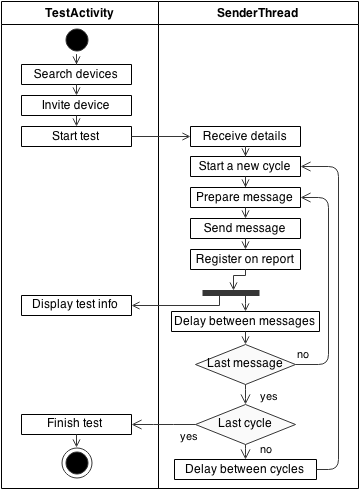
\includegraphics[width=0.40\columnwidth]{testActivityDiagram-BW}
	\caption{PushLoop activity diagram of the test from the sender point of view.}
	\label{fig:pushloopactivityDiagram}
\end{figure}

\begin{figure}[!ht]
	\centering
	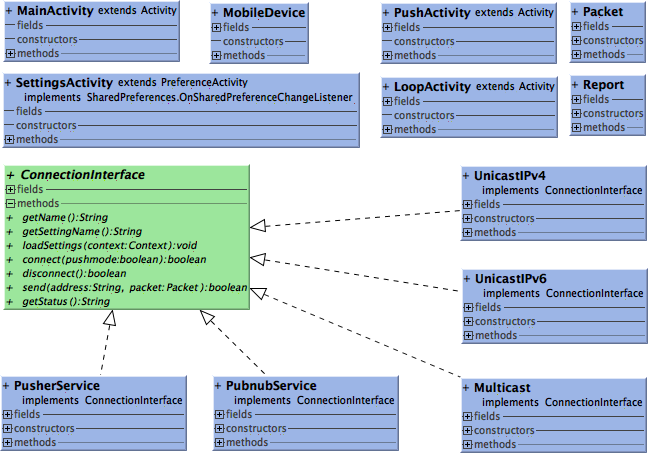
\includegraphics[width=\columnwidth]{PushLoop_ClassDiagram}
	\caption{PushLoop class diagram.}
	\label{fig:pushloopclassdiagram}
\end{figure}

\begin{figure*}[!ht]
	\centering
	\begin{subfigure}{.22\textwidth}
		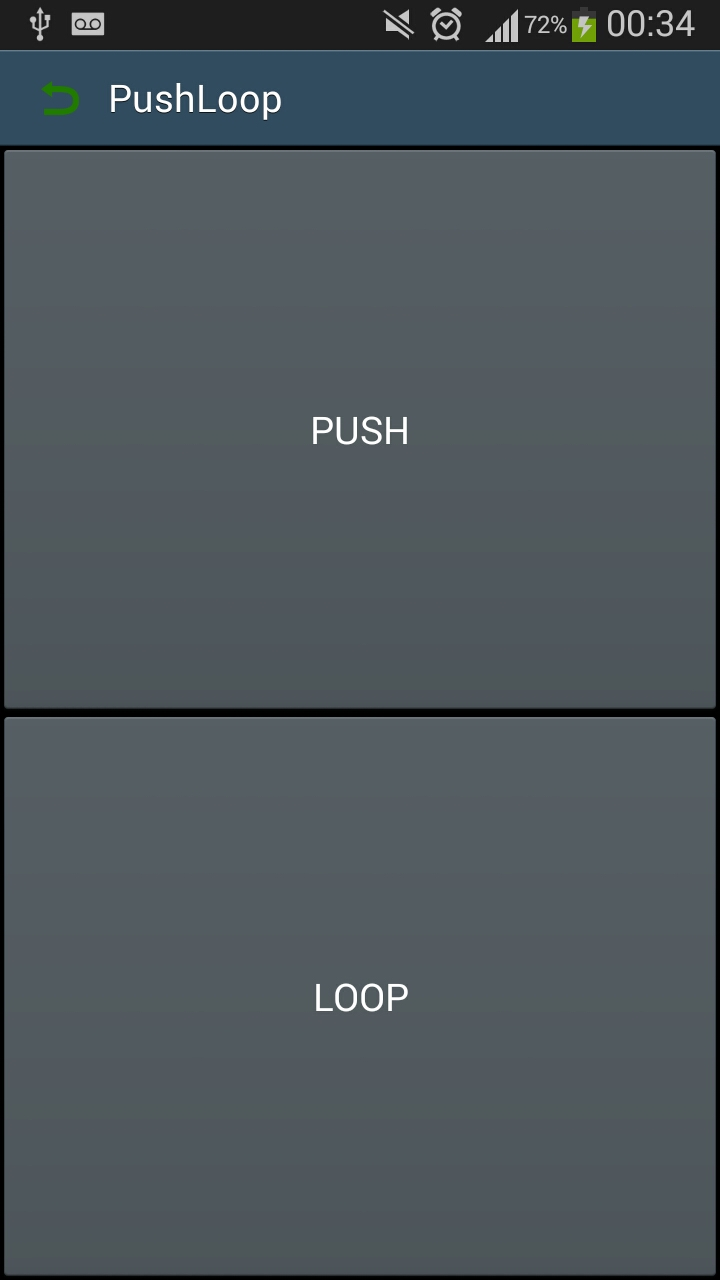
\includegraphics[width=\columnwidth]{pushloop_screenshot}
		\caption{Main screen}
		\label{fig:pushloopss1}
	\end{subfigure}
	\begin{subfigure}{.22\textwidth}
		\centering
		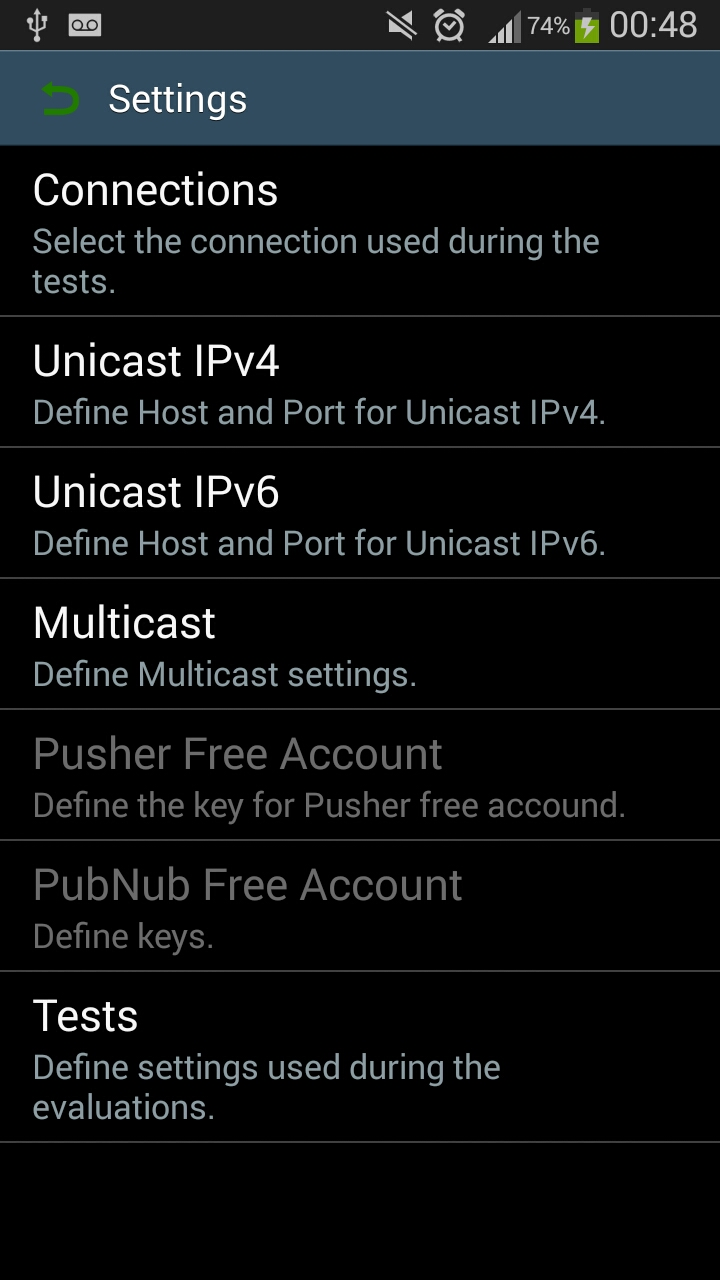
\includegraphics[width=\columnwidth]{pushloop_screenshot2}
		\caption{Setting screen}
		\label{fig:pushloopss2}
	\end{subfigure}
	\begin{subfigure}{.22\textwidth}
		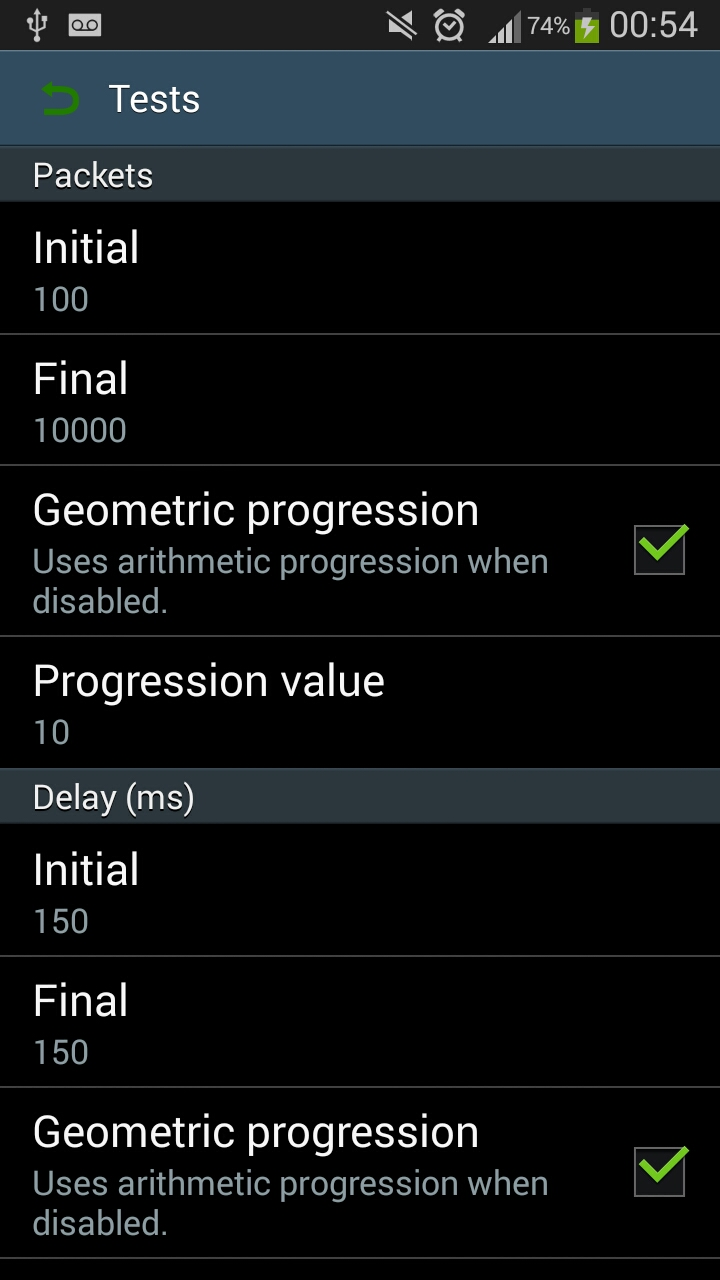
\includegraphics[width=\columnwidth]{pushloop_screenshot3}
		\caption{Test screen (1)}
		\label{fig:pushloopss3}
	\end{subfigure}
	\begin{subfigure}{.22\textwidth}
		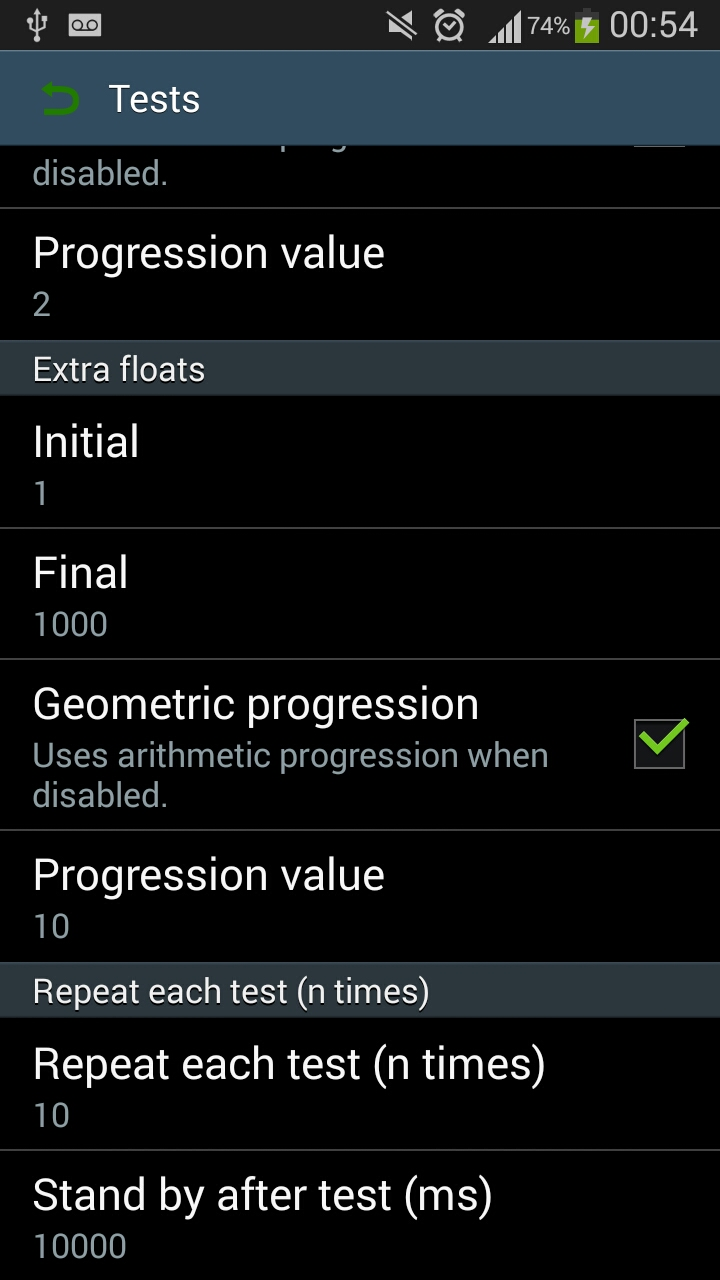
\includegraphics[width=\columnwidth]{pushloop_screenshot4}
		\caption{Test screen (2)}
		\label{fig:pushloopss4}
	\end{subfigure}
	
	\caption{PushLoop application screenshots.}
	\label{fig:pushloopscreenshots}
\end{figure*}

The code of the application is available at \url{https://github.com/deusanyjunior/PushLoop} (visited on May, 2017). 
The first evaluation using this application was published as a paper at the International Computer Music Conference, at Denton, Texas, USA~\citep{deCarvalhoJunior2015computer}.
This paper is presented in Appendix~\ref{ape:papericmc2015}.
Chapter~\ref{cap:evaluations} is based on the evaluations conducted with this application.



%%%%%%%%%%%%%%%%%%
\section{Music Processing}

The mobile music scenarios addressed in this research always considered that audio synthesis and processing took place within mobile devices, and that network communication was mainly used for symbolic and control data. The reasons for this assumption is twofold: on the one hand, previous work at the Computer Music research group at IME/USP already indicated that most Android devices back in 2012 were able to process audio in real-time~\citep{bianchi2014processamento}; on the other hand, latency and jitter in network audio transmission were important factors for mobile devices (mostly connected wirelessly), together with transmission costs due to mobile data plans that also rendered audio streaming less appealing in scenarios with large audiences. Some programming languages specifically designed for music and audio processing running inside mobile devices were at the core of many applications proposed here.


\paragraphdesc{Pure Data}
\paragraphdesc{Csound}
\paragraphdesc{SuperCollider}
Pure Data is the main computer music language used in this research, and is used in the applications described in Appendices~\ref{apesec:appthereminimal}, \ref{apesubsec:appsensors2pd}, and \ref{apesec:apphoketus}.
The CSound language was used for the development of the application \textit{Touches On The Line}, described in Appendix~\ref{apesec:apptouchesontheline}.
SuperCollider was used in the development of the collaborative and cooperative live coding application named \textit{SuperCopair}, which is presented in Appendix~\ref{apesec:appsupercopair}.

\paragraphdesc{Web Audio}
The applications developed for mobile music interaction through a web browser were created using the Web Audio API for audio synthesis.
Appendices~\ref{apesec:appcrowdincloud} and \ref{apesec:appbandaaberta} describe the applications \textit{Crowd in C[loud]} and \textit{Open Band}, respectively, that use Web Audio for music processing.

\paragraphdesc{STK at \textit{urMus}}
During the development of applications for iOS devices, the \textit{urMus} platform was used, where audio synthesis is done using the STK.
Music synthesis can be programmed using flowboxes in the \textit{urMus} interface or with Lua language flowboxes abstractions.

%% ------------------------------------------------------------------------- %%
\section{Scope of the Evaluation Process}\index{methodology of evaluation!scope}
\label{sec:scope}

\paragraphdesc{definition of the scope: past experiences and technological improvements (future)}
Technologies were improving during this research, and while some technologies were getting increasingly popular, such as the 802.11ac wireless standard and Cloud Services, others were hardly used since its conception, such as Multicast data transmission over academic networks and IPv6 sockets.
Some selected technologies were a bet due to the uncertainty of the market, with an expectation that these technologies would become popular in a near future.

\subsection*{Sensors and packet rate}

\paragraphdesc{the delay between packets relation with sensors and touch events}
Android Developer Guide for Sensors\footnote{Android Developer Guide for Sensors: \url{https://developer.android.com/guide/topics/sensors/} (visited on December, 2018)} describes four different sensor rates named as Normal (with a delay of 200~ms between each sample), UI (with 60~ms), Game (with 20~ms), and Fastest (with 0~$\mu$~s, that means the device will get sensor data as fast as possible).
From the experiences with the development of some applications such as the Thereminal~(Appendix~\ref{apesec:appthereminimal}) and Sensors2PD~(Appendix~\ref{apesubsec:appsensors2pd}), the users noticed that most sensor rates work as expected, except the Fastest rate, which displayed an unstable rate.
An evaluation of Android sensors determined the minimum delay between sensor events to be around 5ms for accelerometer at fastest sampling rate~\citep{Ma2013experimental}.

These values express that the maximum frequency is 200~Hz for three float numbers representing the accelerometer coordinates.
For instance, the touch responsiveness of Android devices depends on the screen scan frequency but some circuits can scan at 120~Hz and find up to 10 fingers position, what implies 10 pair of position values on every 8~ms in the best situation~\citep{Padre2017touchresponsiveness}.
Bearing in mind these values, this research process considered the sampling rate varying from 4~Hz to 500~Hz, in order to verify the performance at normal situations and also at fastest ones.  

\subsection*{Packet size}

\paragraphdesc{data size, MTU}
According to the RFC1191~\citep{RFC1191MTU}, the Maximum Transmission Unit~(MTU) is 1500~bytes in most Ethernet Networks.
It means that a packet will be fragmented in case its size is higher than this unit, and the device will need to wait more than one packet to get the full data and interpret the information.
In that sense, the packets sent during the evaluations were defined to carry less than 1500~bytes of data in order to avoid packet fragmentation.

\subsection*{WiFi communication}

\paragraphdesc{wifi standard: Mbps and Gbps}
The WiFi connection was set-up at AC1750 to work only with 802.11a and 802.11ac standards, reaching up to 1Gbps.
Although house clients in Brazil have Internet connection available in Mbps, companies and Brazilian universities can take advantage of Gbps connections (up to 50Gbps).
In the USA, Gbps connections are already offered as home Internet services, and Universities have 100Gbps available.
Considering that the Internet options are getting better with time, the use of gigabit connections in this research is a bet for future MM proposals.

\subsection*{Unicast and Multicast}

\paragraphdesc{the cloud services selected, size of packets, and transmission limits}
Multicast and Unicast were selected to interconnect devices within academic networks in order to take advantage of the predefined routes.
In order to use Unicast, the user needs to know the public IPs of all devices that will exchange messages.
Although public IPv4 is a scarce network resource today, IPv6 is becoming available for more devices.

\subsection*{Cloud Services}

Cloud Services interconnect any device compatible with their APIs.
Pusher and PubNub were the Cloud Services selected for this evaluation, and Pusher presented some restrictions such as 10kB per message and a maximum rate of 10 messages per second per device, while PubNub restricted message exchanging to 32kB per message (but devices can send as many messages as they want).
The size of messages was above the MTU size, but the limit of messages per second of Pusher implied a minimum delay of 100ms between messages during the tests including Pusher.

\paragraphdesc{cloud services setup}
Although we had few steps to set up the cloud services, the limit of messages to be sent each day imposed limits to the whole evaluation process.
As long as we planned many evaluations and we would need to evaluate all services with the same settings in a sequence in order to share similar network conditions, it was necessary to divide the number of evaluations per day depending on the number of messages sent by the cloud service free plan.

The free account at Pusher had an unchangeable configuration that would stop exchanging messages after reaching the daily limit.
It is important to remember that PubNub service has limits on the free plan, but the system avoids blocking the service and sends emails instead (these e-mails included information about the number of messages exchanged and invited the user to change the plan).

\subsection*{Routes}

The routes between universities and the possible location of the cluster used by the Cloud services are presented in Figure~\ref{fig:routes}.
It is important to notice that every message needs to be sent to the cluster before being pushed to its final destination.
This means that every message exchanged between S\~{a}o Paulo and Jo\~{a}o Pessoa passes by the cluster in USA before reaching its destination.
As one of the main route to USA from Jo\~{a}o Pessoa through the RNP network passes by S\~{a}o Paulo, it is also possible that every packet in a route JPA-SAO passes twice through  S\~{a}o Paulo backbone before reaching its destination inside USP.

The routes are undefined from the point of view of the application, but the packet follow the rules available on the routers and backbones.
In case of using Multicast, it is necessary to inform every network manager to set up the rule for this kind of communication.
As this research process interconnected universities from Brazil and USA, network managers from RNP (Brazil), RedCLARA (Latin America), and Internet2 (USA) were contacted lots of time in order to fix the configuration at their side before the experiments.

\begin{figure}[!ht]
	\centering
	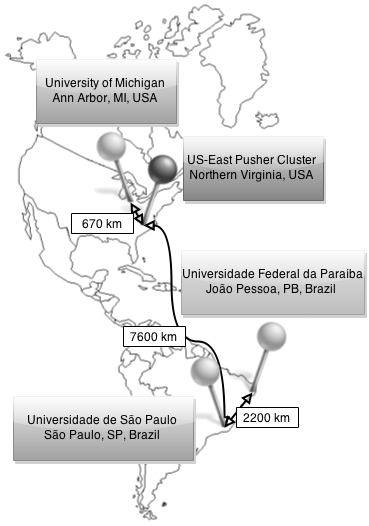
\includegraphics[width=0.4\columnwidth]{evaluation-routes-map-BW}
	\caption{Routes between the universities with linear distance in kilometers}
	\label{fig:routes}
\end{figure}

\subsection*{Evaluation summary}

As this research aimed at many different types of evaluations around the same theme, Mobile Music Technologies, the results for each evaluation and their discussion are presented separately.
The main division of the evaluations is related to the technical or musical aspects.
Although some technical aspects were also discussed in the published papers, the network communication aiming music interaction is described in depth in Chapter~\ref{cap:evaluations} following the scope presented in this Section.
Applications, performances, and music synthesis technologies are briefly discussed in Appendix~\ref{ape:applications}, and an extensive discussion about them is presented in Appendix~\ref{ape:papers}, which contains the papers published in conferences during the research process.

In a nutshell, the evaluation discussed in the next Chapter is based in the following specifications presented below:

\begin{itemize}
	\item The research involved: the University of São Paulo~(USP) at São Paulo, SP, Brazil~(SAO), the Federal University of Paraíba~(UFPB) at João Pessoa, PB, Brazil~(JPA), and the University of Michigan~(UMich) at Ann Arbor, Michigan, USA~(ARB);
	\item The academic gigabit research network infrastructure was used in this evaluation both in Brazil and USA, being the Rede Nacional de Ensino e Pesquisa~(RNP) and Internet2~(I2) responsible for the interconnection within both countries, respectively, while the RedCLARA is responsible for intermediate connection paths between RNP and I2.
	\item LG D686 G Pro Dual Lite~(D686), Samsung GT-I9300 Galaxy SIII~(S3), and Sony D8533 (and D8503) Xperia Z3 Compact~(Z3) were the mobile devices used during the evaluations;
	\item The wireless router TP-Link AC1750 Archer C7 Wireless Dual Band Gigabit Router~(AC1750) used at USP and UMich was set up exclusively for this research, while the AirPort Time Capsule used at UFPB was the available router for users at the Digital Video Applications Lab~(LAViD). Both routers have gigabit connection and are compatible with the 802.11ac wireless standard;
	\item The interconnection between devices was managed through Multicast, Unicast, and Cloud Services;
\end{itemize}

The technologies used during the evaluations related to packet networking are presented in Table~\ref{tab:summarytecheval}.
The evaluations are separated in three experiments with different specifications.
Their specifications are presented in Tables \ref{tab:summaryspeceval1}, \ref{tab:summaryspeceval2}, and \ref{tab:summaryspeceval3}.
These evaluations were managed by the PushLoop application and executed on Android devices.
The results from the First experiment is also discussed in the paper presented in Appendix~\ref{ape:papericmc2015}.

\begin{table}[!ht]
	\centering
	\begin{tabular}{ll}
		\multicolumn{2}{c}{\textbf{Network}} \\ \hline
		\multicolumn{1}{l|}{\begin{tabular}[c]{@{}l@{}}\textbf{Communication} \end{tabular}} & \textbf{Protocols} \\ \hline
		\multicolumn{1}{l|}{Pusher}                                                           & UDP       \\ \hline
		\multicolumn{1}{l|}{PubNub}                                                                  & IPv4      \\ \hline
		\multicolumn{1}{l|}{Unicast}                                                               & IPv6      \\ \hline
	\end{tabular}
	\caption{Summary of Network technologies evaluated in Chapter~\ref{cap:evaluations}.}
	\label{tab:summarytecheval}
\end{table}


\begin{table}[!ht]
	\centering
	\begin{tabular}{l|l|l|l}
		\textbf{Routes} & \textbf{Communication} & \textbf{\begin{tabular}[c]{@{}l@{}}Delay (ms)\\ Between\\ Messages\end{tabular}} & \textbf{\begin{tabular}[c]{@{}l@{}}Messages Size \\ (number of floats)\end{tabular}} \\ \hline
		SAO-JPA         & Pusher                 & 150                                                                              & 1                                                                                                  \\ \cline{1-1} \cline{4-4}
		ARB-JPA         &                        &                                                                                  & 50 \\ \cline{4-4}
		&                        &                                                                                  & 100 \\ \cline{4-4}
		&                        &                                                                                  & 150 \\ \cline{4-4}
		&                        &                                                                                  & 200                 \\ \cline{4-4}
		&                        &                                                                                  & 250 \\ \hline
	\end{tabular}
	\caption{Summary of technical specifications evaluated during the First experiment presented in Section~\ref{sec:firsttrial}.}
	\label{tab:summaryspeceval1}
\end{table}


\begin{table}[!ht]
	\centering
	\begin{tabular}{l|l|l|l}
		\textbf{Routes} & \textbf{Communication} & \textbf{\begin{tabular}[c]{@{}l@{}}Delay (ms)\\ Between\\ Messages\end{tabular}} & \textbf{\begin{tabular}[c]{@{}l@{}}Messages Size \\ (number of floats)\end{tabular}} \\ \hline
		SAO-JPA         & Pusher                 & 150                                                                              & 1\\ \cline{1-1} \cline{4-4}
		ARB-JPA         & Pusher Paid            &                                                                                  & 50 \\ \cline{1-1} \cline{4-4}
		ARB-SAO         & PubNub                 &                                                                                  & 100\\ \cline{4-4}
		& PubNub Paid            &                                                                                  & 150 \\ \cline{4-4}
		& Unicast                &                                                                                  & 200 \\ \cline{4-4}
		&                        &                                                                                  & 250 \\ \hline
	\end{tabular}
	\caption{Summary of technical specifications evaluated during the Second experiment presented in Section~\ref{sec:secondtrial}.}
	\label{tab:summaryspeceval2}
\end{table}


\begin{table}[]
	\centering
	\begin{tabular}{l|l|l|l}
		\textbf{Routes} & \textbf{Communication} & \textbf{\begin{tabular}[c]{@{}l@{}}Delay (ms)\\ Between\\ Messages\end{tabular}} & \textbf{\begin{tabular}[c]{@{}l@{}}Messages Size \\ (number of floats)\end{tabular}} \\ \hline
		SAO-ARB         & Unicast IPv4           & 2                                                                                & 2 \\ \cline{2-4}
		& Unicast IPv6           & 4                                                                                & 4 \\ \cline{3-4}
		&                        & 8                                                                                & 8 \\ \cline{3-4}
		&                        & 16                                                                               & 16  \\ \cline{3-4}
		&                        & 32                                                                               & 32 \\ \cline{3-4}
		&                        & 64                                                                               & 64 \\ \cline{3-4}
		&                        & 128                                                                              & 128 \\ \hline
	\end{tabular}
	\caption{Summary of technical specifications evaluated during the Third experiment presented in Section~\ref{sec:thirdtrial}.}
	\label{tab:summaryspeceval3}
\end{table}


The papers in Appendix~\ref{ape:papers} discuss the evaluation of the technologies presented in Table~\ref{tab:summarytechpapers}.
Other technologies were evaluated during the development of the applications and they are presented in Table~\ref{tab:summarytechapps} and discussed in Appendix~\ref{ape:applications}.


\begin{table}[!ht]
	\centering
	\begin{tabular}{l|l|l}
		\multicolumn{2}{c|}{\textbf{Network}} & \multirow{2}{*}{\textbf{Audio Synthesis}} \\ \cline{1-2}
		\textbf{Communication}   & \textbf{Protocols}  &                                  \\ \hline
		Web Servers     & UDP        & Pure Data                        \\ \hline
		Cloud Services  & IPv4       & Csound                           \\ \cline{1-1} \cline{3-3} 
		Unicast         &            & Super Collider                   \\ \cline{1-1} \cline{3-3} 
		&            & Web Audio                        \\ \hline
	\end{tabular}
	\caption{Summary of technologies evaluated in the papers published during the research and presented in Appendix~\ref{ape:papers}.}
	\label{tab:summarytechpapers}
\end{table}



\begin{table}[!ht]
	\centering
	\begin{tabular}{l|l|l}
		\multicolumn{2}{c|}{\textbf{Network}} & \multirow{2}{*}{\textbf{Audio Synthesis}} \\ \cline{1-2}
		\textbf{Communication}    & \textbf{Protocols} &                                  \\ \hline
		Web Servers      & UDP       & Pure Data                        \\ \hline
		Cloud Services   & mDNS      & Csound                           \\ \cline{1-1} \cline{3-3} 
		Unicast          &           & Super Collider                   \\ \cline{1-1} \cline{3-3} 
		Multicast        &           & Web Audio                        \\ \cline{1-1} \cline{3-3} 
		Broadcast        &           & urMus                            \\ \cline{1-1}
		Bonjour/Zeroconf &           &                                  \\ \hline
	\end{tabular}
	\caption{Summary of technologies evaluated in the applications created during the research process and presented in Appendix~\ref{ape:applications}.}
	\label{tab:summarytechapps}
\end{table}
